\subsection{How a query cracks a cluster map using a kd-tree}
%\subsection{$kd$-tree Data Structure \& Algorithms}
\label{subsec:kdtree_adaptive}

To maintain the information about the clusters we need an appropriate index 
data structure. In our implementation this data structure is a $kd$-tree.
Every node $\mathtt{P}$ in the $kd$-tree is associated with $\mathtt{k}$ 
keys or columns, ($\mathtt{c_1(P), c_2(P),\ldots,c_k(P)}$).
In addition to the $\mathtt{k}$ keys, each node contains one pointer to the
left subtree, $\mathtt{LEFT(P)}$, and one pointer to the right subtree, 
$\mathtt{RIGHT(P)}$. Each node $\mathtt{P}$ is also associated with a
discriminator, $\mathtt{DISC(P)}$, which is an integer between 
$\mathtt{1}$ and $\mathtt{k}$.
The defining order imposed by a $kd$-tree is the following.

\begin{flushleft}
\begin{mydef}
\emph{For any node $\mathtt{P}$ in a $kd$-tree, let $\mathtt{j}$ be the
discriminator $\mathtt{DISC(P)}$, then for any node $\mathtt{Q}$ in 
$\mathtt{LEFT(P)}$, it is true that $\mathtt{c_j(Q) < c_j(P)}$;
likewise, for any node $\mathtt{Q}$ in $\mathtt{RIGHT(P)}$, it is true that
$\mathtt{c_j(Q) > c_j(P)}$.}
\end{mydef}
\end{flushleft}

All nodes of any level $\mathtt{l}$ of the $kd$-tree have the same 
discriminator, which is given by $\mathtt{DISC(l)}$ = $\mathtt{(l\ mod\ k)\ +\ 1}$,
where $\mathtt{l \geq 1}$.

\begin{figure}[t]
\begin{center}
\vspace*{3\baselineskip}
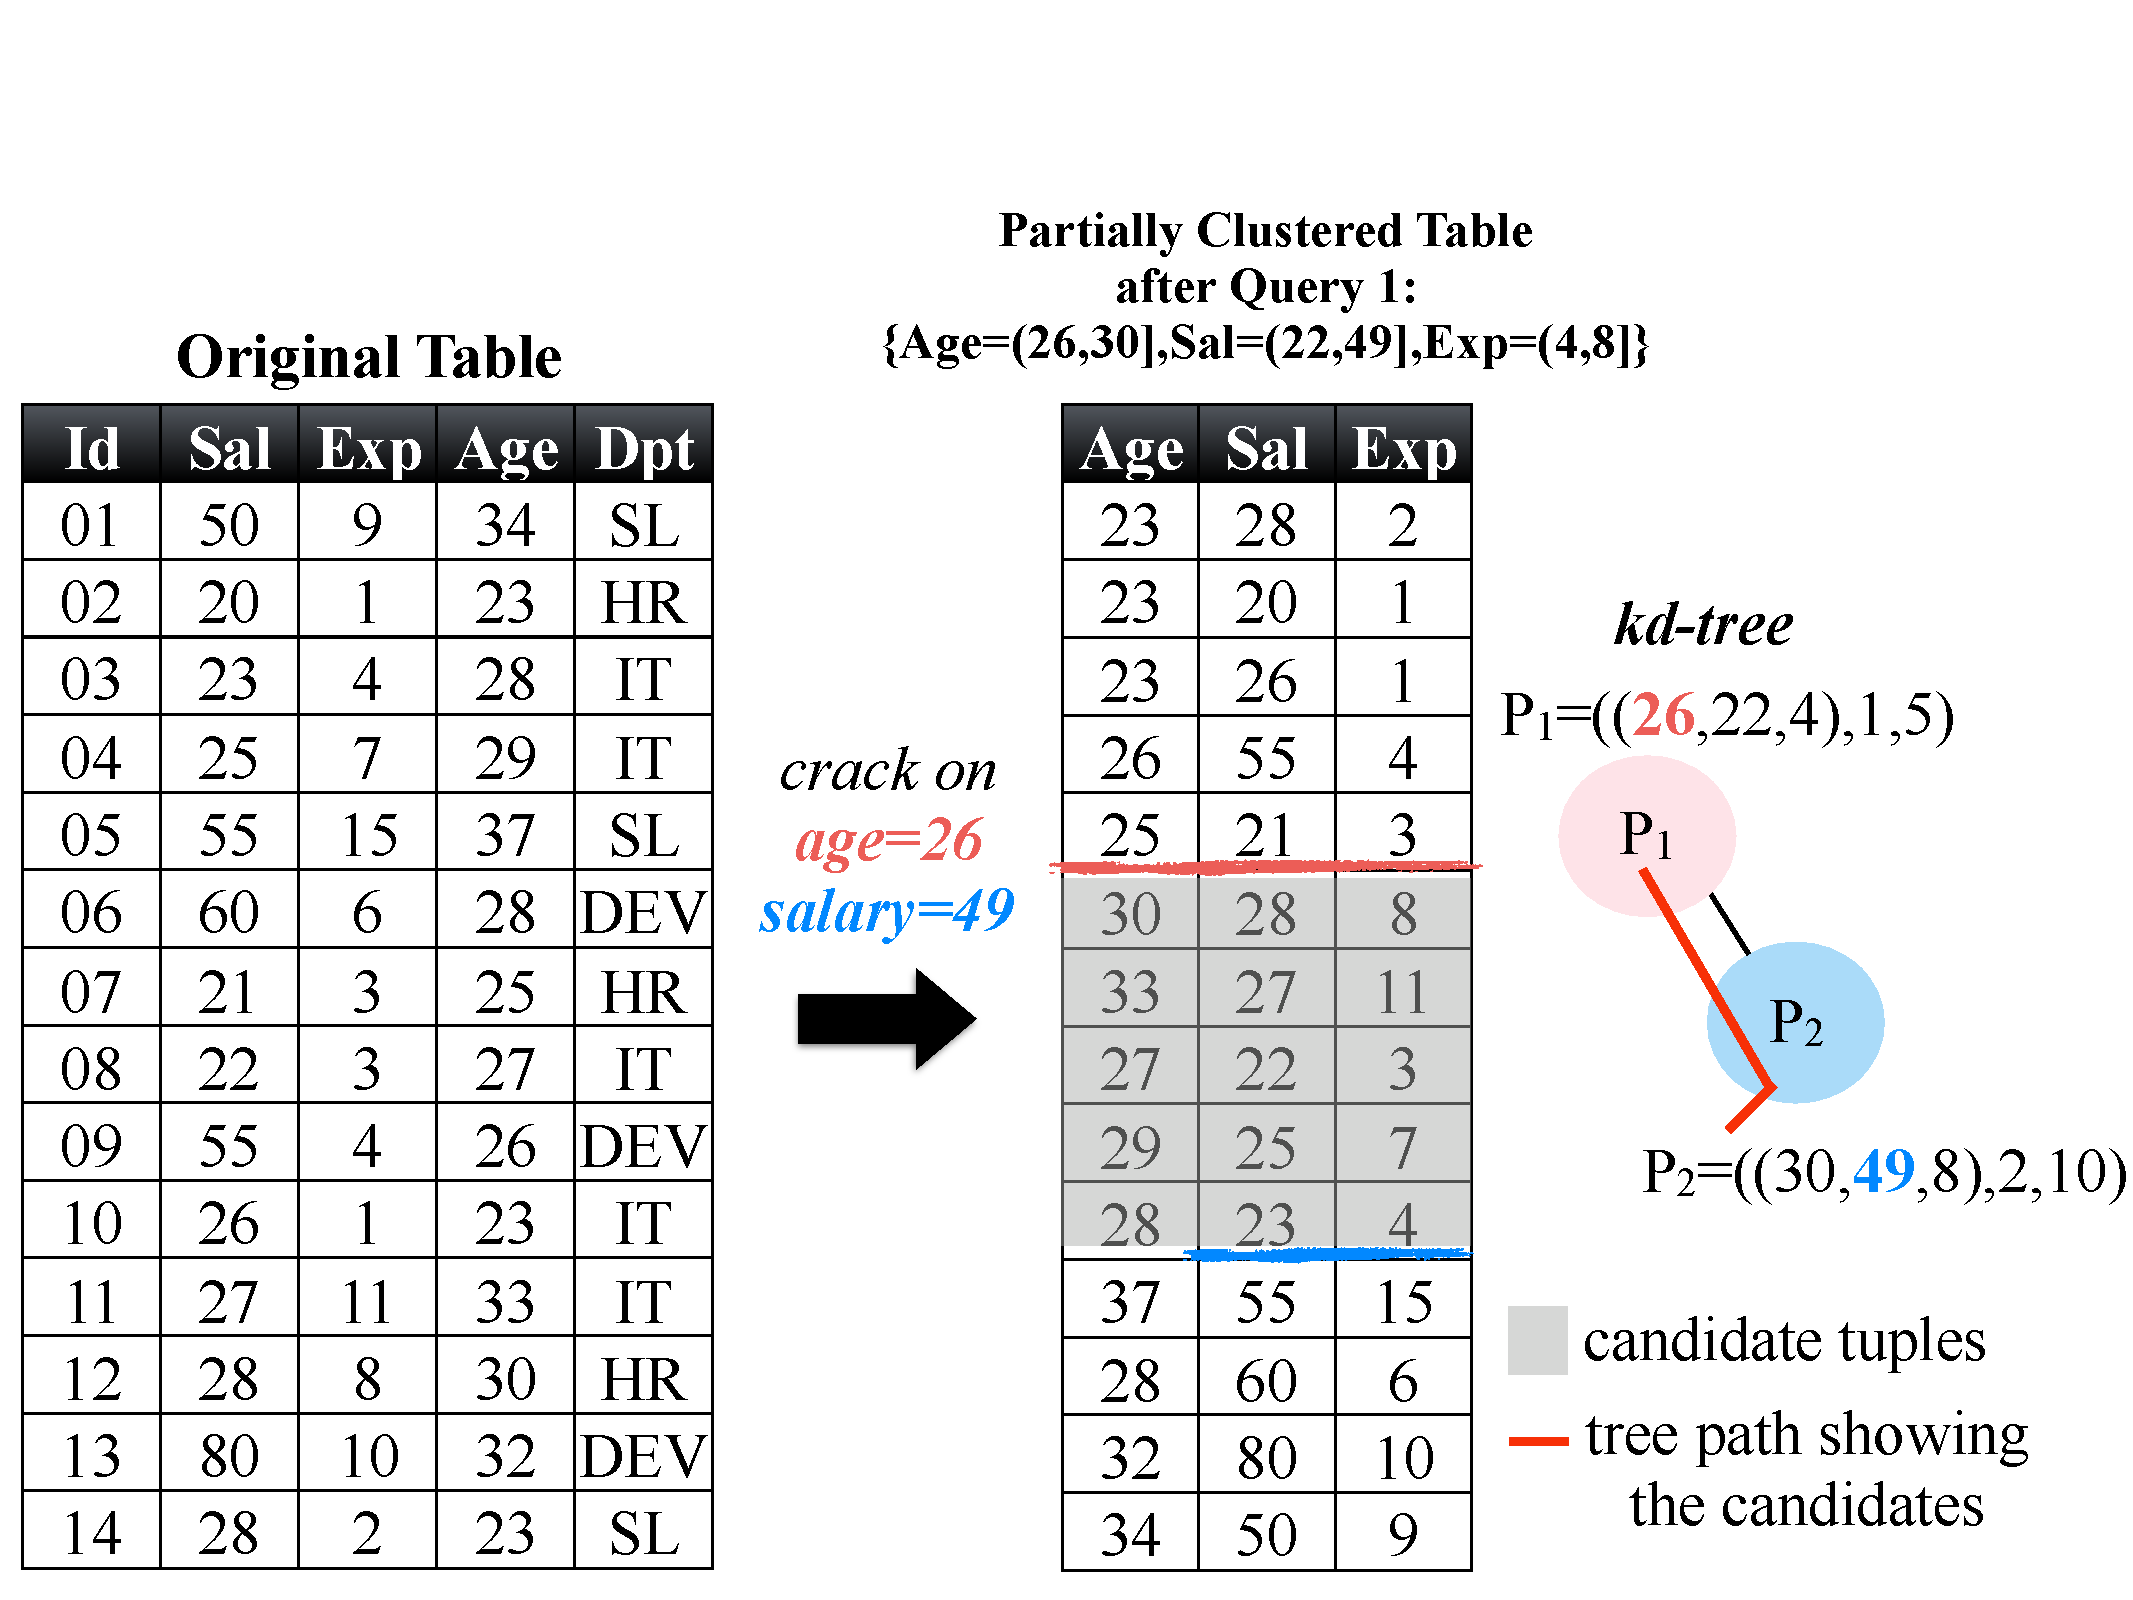
\includegraphics[trim=0cm 2cm 0cm 8.5cm, width=\columnwidth]{Figures/mcrack_kdtree}
\caption{$kd$-tree after the first query.}
\label{fig:pkdtree}
\end{center}
\end{figure}

In adaptive clustering the $\mathtt{k}$ dimensions of a node $\mathtt{P}$ of
the $kd$-tree are associated with query predicates instead of actual data points.

\textbf{Example.}Figure~\ref{fig:pkdtree} shows an example of a $kd$-tree that is built
on the fly during query processing.
The first query 
\begin{center}
$\mathtt{Q^0 = \{Age,Sal,Exp\ |\ Age = (26,31),\ Sal = (22,50),\ Exp = (4,9)\}}$ 
\end{center}
The query consists of two  $\mathtt{k}$-dimensional points, i.e., $\mathtt{(26,22,4)}$ and $\mathtt{(31,50,9)}$.
Before the first query the tree is empty.
The root we will insert to the tree will be in level $\mathtt{1}$, i.e.,  $\mathtt{DISC(root)=1}$, which is associated with dimension ($\mathtt{Age}$).
Thus, we insert in the tree the first point $\mathtt{(26,22,4)}$ which indicates that we need to crack the data on $\mathtt{Age=26}$.
Cracking $\mathtt{Age}$ results in two new partitions, one from positions 0 to 4 and one from positions 5 to 13.
The split position 5 is also inserted in the root node.
The left subtree of the root represents the partition that contains all data points $\mathtt{P}$ with $\mathtt{Age \geq 26}$, while the right subtree represents the partition that contains all data points $\mathtt{P}$ with $\mathtt{Age > 26}$.

To insert the second point $\mathtt{P=(31,50,9)}$ in the tree, we start from the root comparing the value of dimension $\mathtt{Age}$.
Since $\mathtt{31 > 26}$, we are directed to the right subtree, which is empty.
Thus, we can insert the new point $\mathtt{P=(31,50,9)}$ as a right child of the root.
The new point is inserted in level $\mathtt{2}$, i.e.,  $\mathtt{DISC(P)=2}$, which is associated with dimension ($\mathtt{Salary}$).
That information indicates us that we need to crack the partition from position 5 to 13 on $\mathtt{Sal=50}$.
After cracking on  $\mathtt{Sal=50}$, we create two new partitions, one from position 5 to 9 and one from position 10 to 13.
The split position 10 is also added to the new node.

With the above example we showed that every node is associated not only with one of the $k$ dimensions of a query, 
but also with the partitions the query introduces.
The splitting position is the first position of the partition that contains values greater than the value of the cracked dimension.
The split positions stored in the tree nodes indicate the start and end position of the candidate list.
In our example, the data between positions 5 and 10 contains candidate qualifying tuples, which we need to scan in order to retrieve the final result.
Algorithm~\ref{alg:updatePositions} describes how we can retrieve the start and end position of the candidate list by following the tree path to a specific node.

\algsetup{linenosize=\small,linenodelimiter=.}
\begin{algorithm}[t] 
\caption{Update positions[]: update array with predescendant positions}
\textbf{Input: } positions[], newposition, type

\label{alg:updatePositions}
\begin{algorithmic}[1]
\IF { ($type \equiv 'l'$) }
\STATE positions[2] = positions[1]
\STATE positions[1] = newposition
\ELSE
\STATE positions[0] = positions[1]
\STATE positions[1] = newposition
\ENDIF
\end{algorithmic}
\end{algorithm}

To process a subsequent query, we navigate through the $kd$-tree to a node.
If the point stored in the node where we end up is the same as the query, 
that means that the query has already been processed in the past and we need to take some actions in order to return the qualifying tuples. 
If we end up to a null node, we need first to partition the underlying data.
Figure~\ref{fig:kdtree_cracking_two} shows the $kd$-tree after processing the second query
\begin{center}
$\mathtt{Q^1 = \{Age,Sal,Exp\ |\ Age = (24,29),\ Sal = (21,57),\ Exp = (2,8)\}}$.
\end{center}
For this query two points need to be inserted in the tree, i.e., $\mathtt{(24,21,2)}$ and $\mathtt{(29,57,8)}$.
First, we search the $kd$-tree for point $\mathtt{(24,21,2)}$ starting from the root and alternating the dimensions according to the level.
The root is in level $\mathtt{0}$, thus, we compare $\mathtt{Age(root)=26}$ with $\mathtt{Age(Q_1)=24}$.
$\mathtt{Age(Q_1)}$ is less than $\mathtt{Age(root)}$, thus we move to the left child of the root, which is null.
Since the node we ended up is null, i.e., it's the first time we process this query, we partition the data from position 0 to position 4 into two new partitions; the first partition starts from position 0 and ends at position 1 and contains all points $\mathtt{P}$ with $\mathtt{Age(P) \leq 26 \& Age(P) \leq 24}$ , while the second partition starts from position 2 and ends at position 4 and contains all points $\mathtt{P}$ with $\mathtt{Age(P) \leq 26 \& Age(P) > 24}$.
We store position 2 as the node split position.

\begin{figure}[t]
\begin{center}
\vspace*{3\baselineskip}
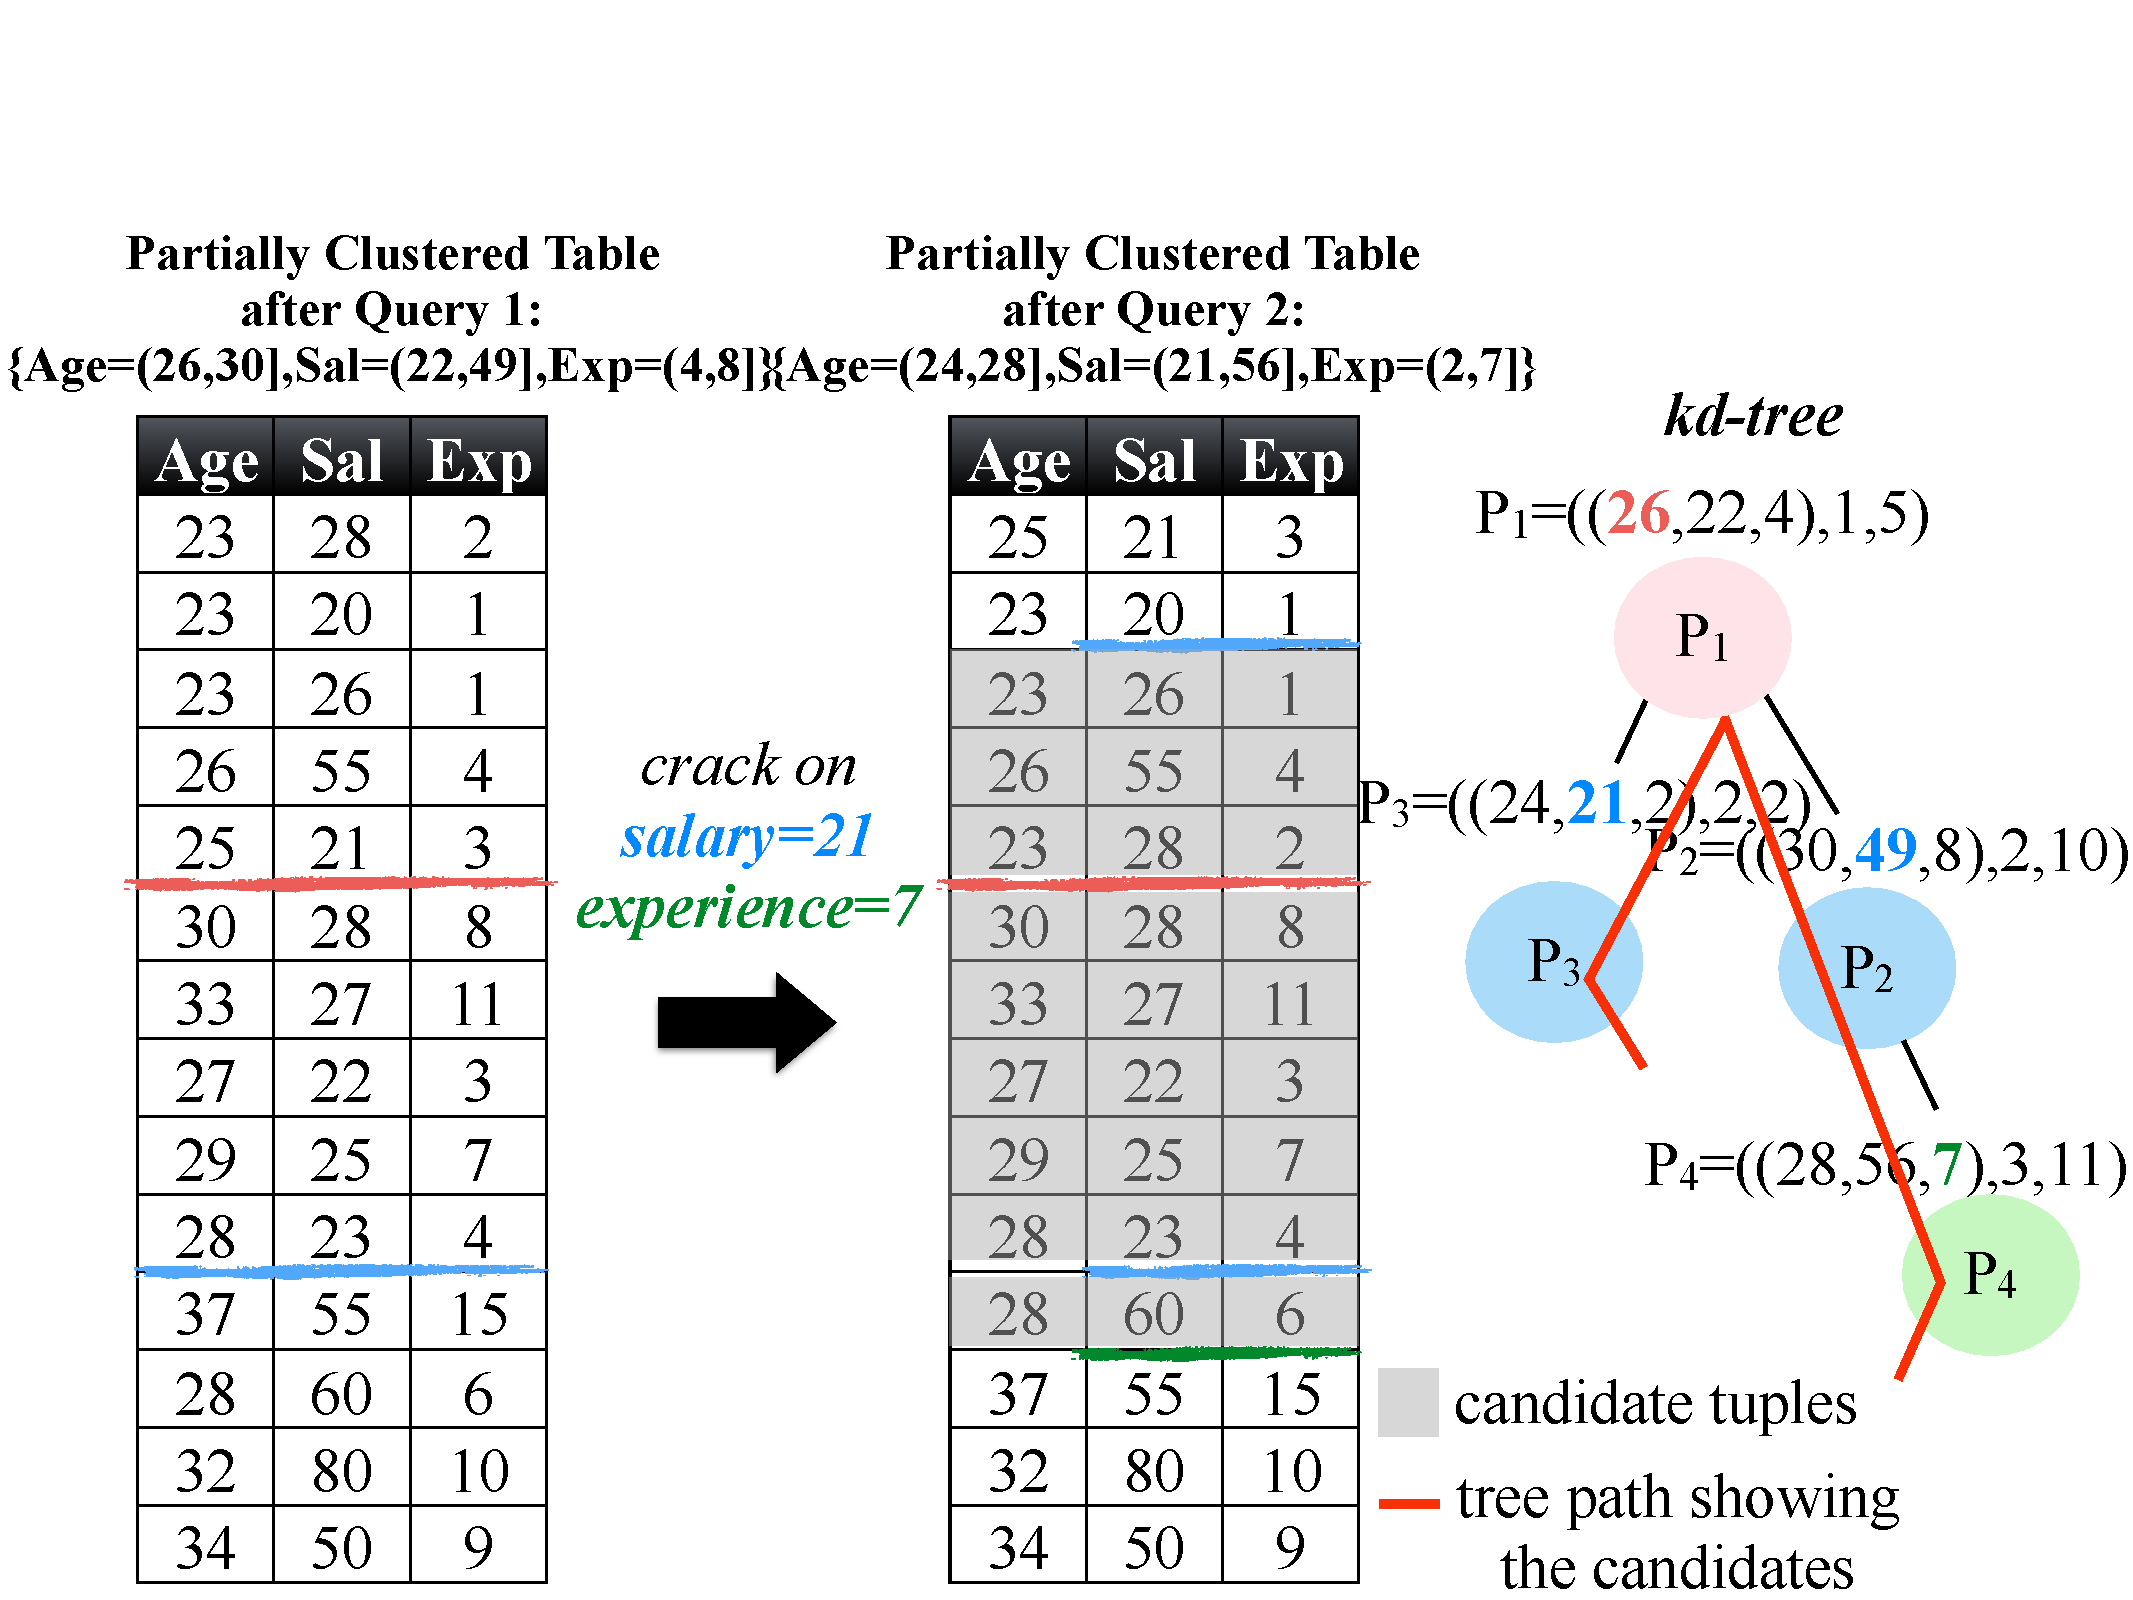
\includegraphics[trim=0cm 2cm 0cm 8.5cm, width=\columnwidth]{Figures/mcrack_kdtree_2nd}
\caption{$kd$-tree after the first query.}
\label{fig:pkdtree}
\end{center}
\end{figure}


We define the following structure to store and administer the KDTree index.

\lstset{language=C}
\begin{lstlisting}
typedef struct kdnode {
	int              *kpoint;
	long              pos;
        struct kdnode    *left;
        struct kdnode    *right;
} kdnode;
\end{lstlisting}

Algorithm~\ref{alg:insertKDTree} describes the steps we follow to insert a new node in the $kd$-tree.


\algsetup{linenosize=\small,linenodelimiter=.}
\begin{algorithm}[t] 
\caption{Insert k-dimensional point in KDTree: insertKDTree()}
\textbf{Input: }KDTree rooted at $root$, $k$-dimensional $point$, number of dimensions $k$ \newline
\textbf{Output: }Inserted Node

\label{alg:insertKDTree}
\begin{algorithmic}[1]
\STATE kdnode $current$ = $root$ %\COMMENT{begin search from root}
\STATE kdnode $previous$ = $NULL$ 
\STATE $levelmod$ = 0
\STATE $type$ =$''$
%\IF [kdtree is empty] { ($root \equiv NULL$) }
\IF { ($root \equiv NULL$) }
\STATE $root$ = newKDNode %\COMMENT{insert new node}
\STATE $root.pos$ = \textbf{crack} from $0$ to $ntuples-1$%\COMMENT{first (out-of-place) cracking}
\ENDIF
\STATE $positions[3]$ = $\{0, root->pos, ntuples\}$
\WHILE { ($current$)}
\IF { ($kpoint \equiv current.kpoint$) }
\STATE return $current$
\ENDIF
\STATE $previous$ = $current$
\IF { ($kpoint[levelmod] < current.kpoint[levelmod]$) }
\STATE $current$ = $current.left$ %\COMMENT{visit left child}
\STATE $type$ = $'l'$
\IF { ($root \ne NULL$) }
\STATE updatePositions($positions,cur.pos,type$)
\ENDIF
\ELSE
\STATE $current$ = $current.right$ %\COMMENT{visit right child}
\STATE $type$ = $'r'$
\IF { ($root \ne NULL$) }
\STATE updatePositions($positions,cur.pos,type$)
\ENDIF
\ENDIF
\STATE $levelmod$ = ($levelmod$ + 1) \% $k$
\ENDWHILE
\IF { ($type \equiv 'l'$) }
\STATE $previous.right$ = newKDNode
\STATE $previous.left.pos$ = \textbf{crack} from $positions[0]$ to $positions[1]-1$ %\COMMENT{(in-place) cracking}
\STATE return $previous.left$
\ELSE
\STATE $previous.right$ = newKDNode
\STATE $previous.right.pos$ = \textbf{crack}  from $positions[1]$ to $positions[2]-1$ %\COMMENT{(in-place) cracking}
\STATE return $previous.right$
\ENDIF
\end{algorithmic}
\end{algorithm}


Algorithm~\ref{alg:answerQ} describes the steps we follow to select the qualifying tuples of a query of the form we described in ~\ref{sec:Introduction}.


\algsetup{linenosize=\small,linenodelimiter=.}
\begin{algorithm}[t] 
\caption{Search for qualifying tuples: selectKDTree()}
\textbf{Input: }KDTree rooted at $root$, $k$-dimensional $minpoint$ with query minimum boundaries, $k$-dimensional $maxpoint$  with query maximum boundaries, number of dimensions $k$ \newline
\textbf{Output: }Qualifying typles

\label{alg:answerQ}
\begin{algorithmic}[1]
\STATE $root$ = insertKDTree($root, minpoint, \&scanstart$)
\STATE $root$ = insertKDTree($root, maxpoint, \&scanend$)
\STATE Scan data from $scanstart$ to $scanend$
\end{algorithmic}
\end{algorithm}




